\pdfoutput=1
\documentclass[11pt]{article}

% Change "review" to "final" to generate the final (sometimes called camera-ready) version.
% Change to "preprint" to generate a non-anonymous version with page numbers.
\usepackage[review]{acl}

\usepackage{times}
\usepackage{latexsym}
\usepackage{amsmath} 
\usepackage{subfigure}
\usepackage{booktabs}
\usepackage{hyperref}
\usepackage{authblk}
\usepackage{listings}
\usepackage{float}
\usepackage[T1]{fontenc}
\usepackage{microtype}
\usepackage{inconsolata}
\usepackage{graphicx}

\title{Topic Segmentation Using Generative Language Models}

\author{
 \textbf{Pierrre Mackenzie}$^{\star,\dagger}$,
 \textbf{Maya Shah}$^{\star,\ddagger}$,
 \textbf{Patrick Frenett}$^{\star}$,
\\
 $^\star$Adarga,
 $^\dagger$University of Edinburgh,
 $^\ddagger$University of Exeter,
\\
 \small{
   \textbf{Correspondence:} \texttt{lardet[dot]pierre[at]gmail.com}
 }
}

\begin{document}
\maketitle
\begin{abstract}
      Topic segmentation using generative Large Language Models (LLMs) remains relatively unexplored. Previous methods use lexical or semantic similarity between parts of a document to decide on boundaries but they lack the long range dependency and vast knowledge contained in LLMs. In this work we propose a new prompting strategy and compare to methods based on semantic similarity. We also support the adoption of a less commonly used evaluation metric: Boundary Similarity. Results show that LLMs can be more effective segmenters than existing methods, but issues remain to be solved before they can be relied upon for topic segmentation.
  \end{abstract}

\section{Introduction}

% 1
% ---------- Introduction ----------
% 1.1 Motivation
\subsection{Motivation}

% Topic segmentation can be important as a pre-processing step before some other NLP task, or can be important in its own right. 

Tasks such as information retrieval, long-document summarisation and classification can all benefit from first being broken down by topic. For many open source or resource-constrained models, context windows limit the size of input. Although context windows can be increased~\cite{ExtendingContextWindows} and newer models have long context windows, LLMs do not fully utilise long context windows~\cite{EffectOfLongContextWindows,ContextAffectsFactual}.

Furthermore, segmentation can be imporant for its own sake. One might use segments to generate a contents page for a long document or create summaries of parts of a document. Alternatively, one might use segmentation to break down a long document into smaller parts for a user to read or as input in RAG~\cite{RAG}, in which the model must generate an answer to a question based on a segment of text.

% Our application of interest is to use topic segmentation as both a pre-processing step for a document understanding pipeline and as an important step in its own right. This pipeline is used to extract structured information from unstructured text, and the segmentation step is used to break down the document into smaller, more manageable parts. When presented to a user, only semantically self-contained sections of a long document are presented to a user, which can be more easily understood and acted upon.
% 1. Introduction
% 1.1 Topic Segmentation Task Definition

\subsection{Task Definition}

% We can interpret segmentation as a binary classification task.  Given a list of input sentences $S$, of length $n$, the model must decide whether there exists a segment boundary between each pair of adjacent sentences. There are $n-1$ possible boundaries, and therefore the solution space is $2^{n-1}$.  Formally, the model must find a mapping $f$ from the list of sentences to a binary vector of length $n-1$:
% \(
%      f(S) = \textbf{y} 
% \)
% \( \textnormal{ where } \textbf{y}=\{y_1,y_2\ldots,y_{n+1}\} \textnormal{ and each of the } y_i\in\{0,1\}.
% \)

% Relative to generative tasks such as summarisation, the space of possible solutions is much smaller, but the problem remains subjective as where a boundary should lie can be ambiguous. Frequently, humans cannot agree on a correct solution \cite{TextTiling}.

Topic segmentation is the problem of dividing a string of text into constituent `segments'. Each segment should be semantically self-contained such that it is about one thing. The precise definition of a segment is vague and dependent upon the specific use case. For this work, segment boundaries always lie on sentence boundaries. We can then interpret segmentation as a binary classification task: given a list of input sentences of length, the model must decide whether there exists a boundary between each pair of adjacent sentences. While the solution space is smaller than generative tasks, the problem is subjective as frequently humans cannot agree on a segmentation \cite{TextTiling}.



 

\begin{figure*}[t]
    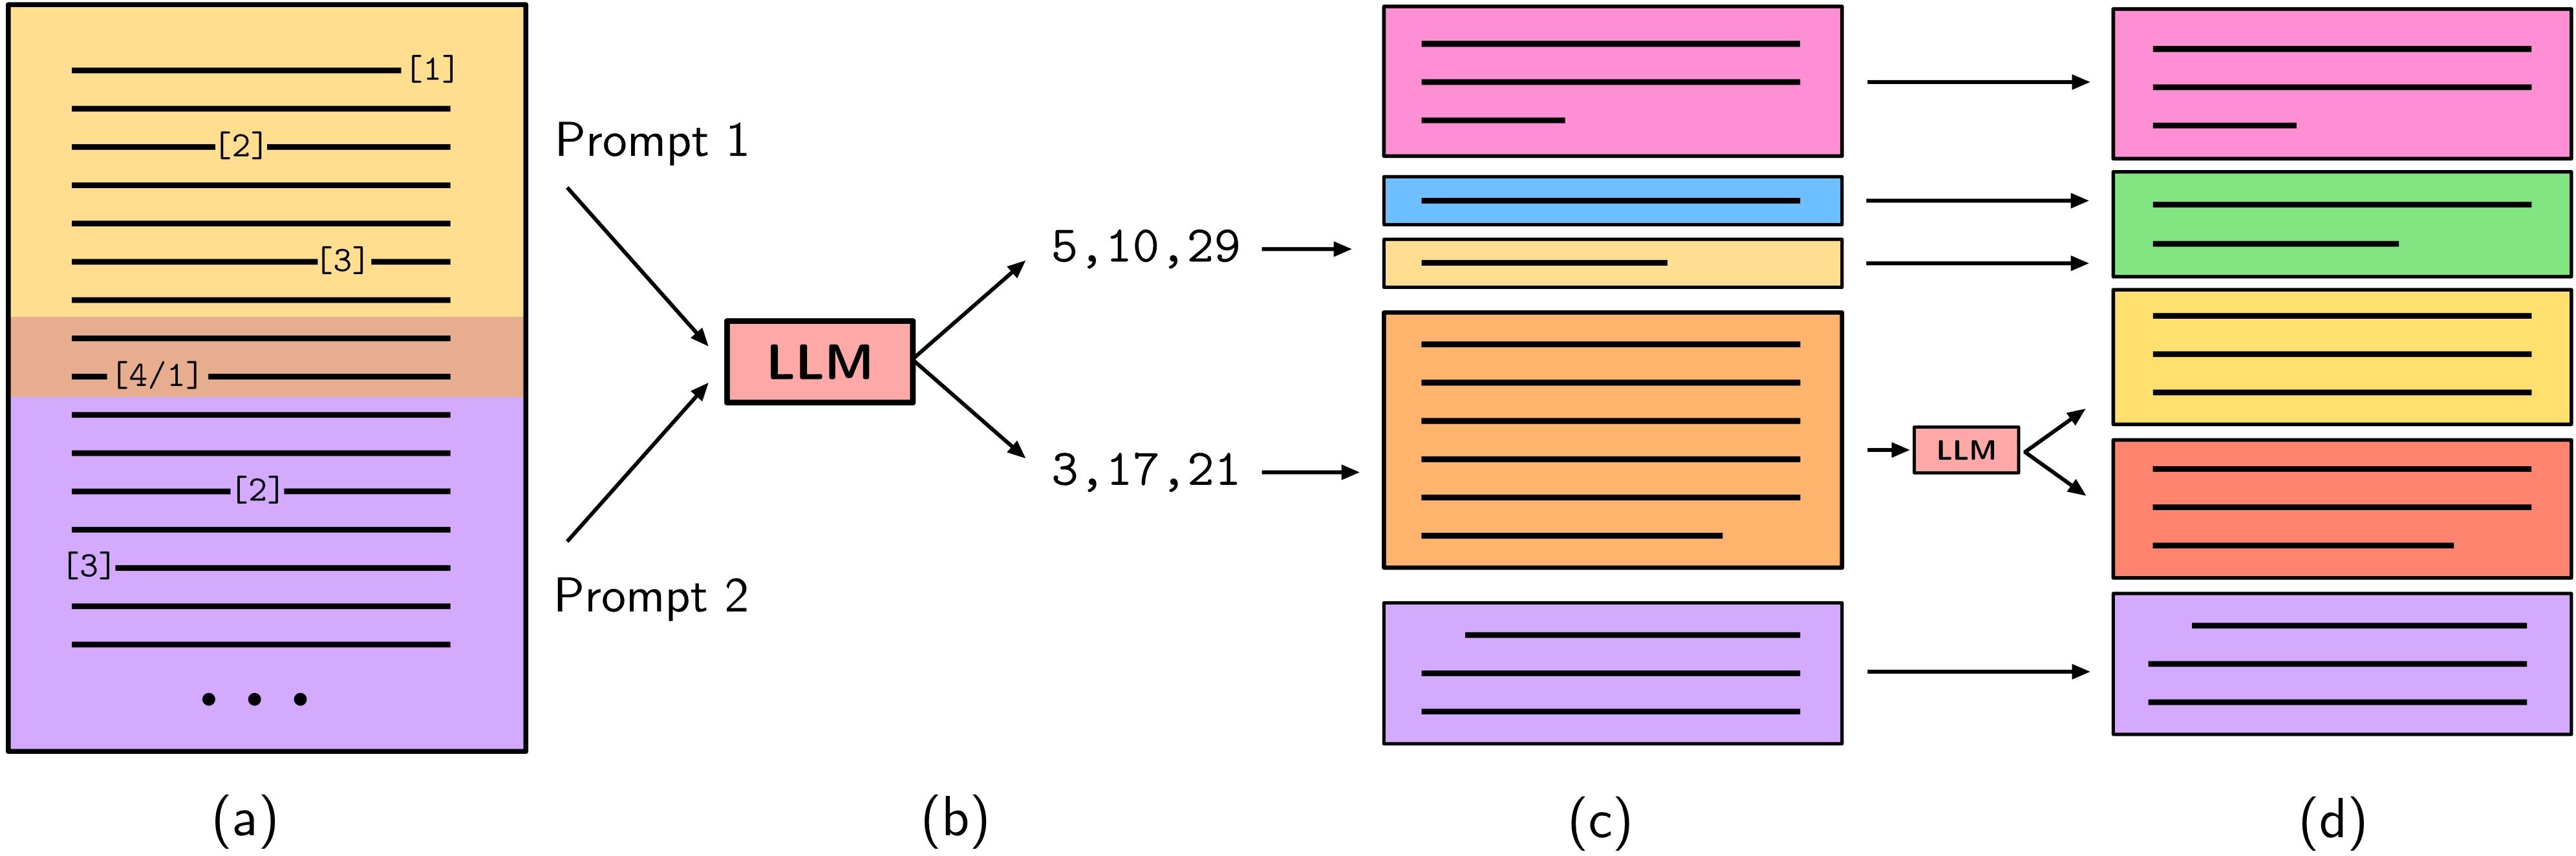
\includegraphics[width=\textwidth]{assets/diagram.png}
    \caption{The overlapping and recursive prompting strategy for segmentation. In (a), a long document is split into overlapping sections with sentence boundaries enumerated. In (b), each section is segmented by the LLM. In (c), the segments are joined. Finally, in (d), each segment is validated to ensure it is not too long or too short.}~\label{fig:diagram}
    \vspace{-2em}
  \end{figure*}
\subsection{Related Work}

Please refer to \citep{XingThesis} which provides a recent, broad overview of topic segmentation.

An influential framework introduced by~\citep{TextTiling} involves computing lexical similarity scores between adjacent sentences before boundaries are placed where similarity is lowest~\citep{lexical1,lexical2}. Such a framework is still in use today but with semantic similarity calculated from embeddings. Neural networks have seen use as BiLSTMs ~\citep{BiLSTM,HierarchicalBiLSTM,CNNFeaturesLSTMAttention} and attention-based methods~\cite{CrossAttentionHierarchical,TwoLevelTransformerSoftmax,TwoLevelTransformerPretrained}. However, these models do not leverage the vast knowledge contained in the largest pre-trained models.

LLMs are the state of the art for a variety of NLP tasks. However, there has been little research into their use for topic segmentation. A loss-based approach was proposed by~\citep{DialoGPT} in which boundaries are placed at peaks in the mean negative log likelihood of tokens in a sentence, indicating that the sentence was hard to predict. This method relies on the dubious assumption that all information about segment boundary location can be expressed by the next token prediction loss.

Previous work has explored segmentation by prompting LLMs~\citep{XingThesis}. They find that prompting ChatGPT is the best dialogue segmentation model unless the input exceeds ChatGPT's limit. Two prompting methods are proposed: one which asks the LLM to return the original text with characters delimiting boundaries and a second in which the LLM is asked to return semantic coherence scores for each pair of sentences. The first method does not satisfy a guarantee that the model will return the original document unedited and is massively wasteful of tokens. In the second method, the returned scores have no guarantee of directly corresponding to semantic coherence specifically for topic segmentation. We propose a new prompting method that ensures the output text is unedited, is much more token-efficient, and is not limited by the context window of the model. We show that this outperforms existing non-prompting based approaches by comparing to our own existing method which uses SentenceBERT embeddings and cosine similarity.

% \vspace{-0.2em}
\begin{table*}[t]
    \centering
    \begin{tabular}{@{}lcccc@{\hspace{2em}}ccccc@{\hspace{0.2em}}c@{}}
    \toprule
    & \multicolumn{4}{c}{Boundary Similarity ($n=2$)} & \multicolumn{6}{c}{Boundary Precision and Recall} \\ 
    \midrule
    & Human & Wiki & Conc-Wiki & Synthetic & \multicolumn{2}{c}{Human} & \multicolumn{2}{c}{Wiki} & \multicolumn{2}{c}{Conc-Wiki} \\ 
    &  &  &  &  & BP & BR & BP & BR & BP & BR \\
    \midrule
    \it GPT3.5  & \bf 0.38 & \bf 0.25 & 0.29 & \bf 0.35 & \bf 0.51 & \bf 0.60 & 0.36 & \bf 0.55 & 0.42 & \bf 0.63 \\ 
    \it FlanT5  & 0.25 & 0.24 & 0.41 & 0.33 & 0.38 & 0.46 & \bf 0.43 & 0.37 & 0.65 & \bf 0.63 \\ 
    \midrule
    \it BERTGraph   & 0.20 & 0.15 & 0.45 & 0.21 & 0.47 & 0.25 & 0.39 & 0.21 & 0.79 & 0.54 \\ 
    \it BERT    & 0.18 & 0.09 & \bf 0.46 & 0.18 & 0.33 & 0.39 & 0.23 & 0.37 & \bf 0.91 & 0.50 \\ 
    \it RandomF0.1 & 0.09 & 0.11 & 0.10 & 0.10 & 0.16 & 0.21 & 0.34 & 0.16 & 0.20 & 0.16 \\ 
    \it Split5  & 0.13 & 0.19 & 0.19 & 0.23 & 0.17 & 0.48 & 0.33 & 0.39 & 0.25 & 0.52 \\ 
    \bottomrule
    \end{tabular}
    \caption{Mean Boundary Similarity, Precision (BP) and Recall (BR) with $n=2$ for each model and dataset.}~\label{tab:combined_results}
    \vspace{-2em}
\end{table*}


% 2
% ---------- Method ----------
\section{Method}
% 2. Method
% 2.1 Datasets
\subsection{Datasets}

There are 4 types of datasets used in the experiments in this work: a small human-annotated dataset, a scrape of English wikipedia, a 'concatenated' wikipedia scrape and a synthetic GPT3.5 generated dataset.

\subsubsection{Human-Annotated Dataset}

Lacking the resources to create a large dataset annotated by humans, this work uses a very small manually segmented dataset of 10 documents. These documents are a mix of news articles, wikipedia articles, and miscellaneous documents such as podcast transcripts and scientific reports. This was intended to represent varying difficulties of segmentation, and provide examples which could be manually inspected to interpret segmenter behaviour. Only one annotator was used, and the segments were created by hand. Further work might involve multiple annotators on a much larger dataset, with a more rigorous process to ensure consistency and quality.

\subsubsection{Wikipedia Dataset}

A plain text English wikipedia scrape\footnote{\url{https://www.kaggle.com/datasets/ltcmdrdata/plain-text-wikipedia-202011/data}} was used articles where headings were delimited by special characters. The articles were then automatically segmented based on headings, and filtered to remove articles with very few segments, too short segments, or too much punctuation such as tables and figures. After this process, there remained approximately 1000 segmented articles. We generate two version of this dataset: one with headings removed, and one with headings included. This was used during evaluation to investigate if a model is merely segmenting based on headings.

\subsubsection{Concatenated Wikipedia Dataset}

We randomly sampled segments from the previous Wikipedia dataset and concatenated them in order to form new incoherent articles, with segments drawn from completely different domains. Intuitively, this dataset should be easier to segment as there are no semantic links between segments.

\subsubsection{Synthetic Dataset}

The final dataset used was generated synthetically by GPT-3.5. The source data was a mix of CTC sentinel data\footnote{\url{https://ctc.westpoint.edu/ctc-sentinel/}}, UN-Peacekeeping corpus\footnote{\url{https://peacekeeping.un.org/en/reports}} and an internal dataset at Adarga. These documents were segmented by querying OpenAI's API with the model \texttt{gpt-3.5-turbo-16k} using the overlapping prompt schema defined in section~\ref{LLM-Based Text Segmentation}. This dataset was exclusively used for fine-tuning the \emph{FlanT5}\ref{FlanT5} model. It was not used for evaluation as the results would be biased in favor of the generative models.
% 2. Method
% 2.2 Evaluation
\subsection{Evaluation}\label{evaluation}

We follow the work in~\cite{fournier-2013-B} which proposes the Boundary Similarity metric and associated precision/recall. The metric pairs segment boundaries between a hypothesised and references segmentation. Exact matches score 1 and no match scores 0, whilst matches within a distance $n$ score linearly in the distance. Boundary Similarity (B) is the mean score, while Boundary Precision/Recall (BP/BR) are the mean score of matched hypothesis/reference boundaries, respectively. For further justification for the use of boundary similarity as opposed to more traditional metrics such as WD and Pk~\cite{HearstW2002}, see~\cite{fournier-2013-B}, or our own investigations\footnote{\url{https://github.com/PierreRL/segmenter-evaluation-metrics}}.

% or our own investigations at \href{https://github.com/PierreRL/segmenter-evaluation-metrics}{segmenter evaluation metrics}.
% 2. Method

\subsection{LLM-Based Text Segmentation}\label{LLM-Based Text Segmentation}

% 2.3 LLM-Based Text Segmentation

How can we get LLMs to output segment boundaries?

We might first consider passing in the input text as a prompt and asking the LLM to copy out the text, adding markers indicating where it has placed boundaries as is suggested by~\citep{XingThesis}. However, not only is this wasteful of tokens, especially if the input text is long, but crucially, the GLM may fail to copy the input accurately, may change the formatting, and we found through qualitative experimentation that boundary placement was not any better than our final method. These problems are addressed by~\citep{XingThesis} through repeated prompting until the input and output sequence lengths match, but this still does not guarantee integrity of the data. In our use case, guaranteeing that the input data would remain the same was of the utmost importance, so we used a different strategy.

\subsubsection{Prompting Method}

We first annotate the text with indices between each sentence. Here is an example: `Hello World. [1] The sky is blue. [2] The sun is is yellow. [3] The grass is green. [4] Machine learning is a rapidly evolving field'. We then ask the LLM to return a list of indices corresponding to boundaries. In the previous example, the ideal response might be `1,4'. In practice, the texts and list of segment boundaries are much longer.

We add a system prompt which describes the segmentation task, desired output format and primes the model to be a talented linguist. We also add a variety of short examples in line with the few-shot prompting technique~\citep{FewShotLearners}, which improved performance. This did not necessarily reflect the fact that the LLM learned how to segment better. Instead, through manual testing, we suspect that it learned the ideal segment length and amount of information that should be contained within a segment, which was implicitly contained in the few-shot prompt (and also the testing datasets, therefore increasing performance). This suggests that different implicit definitions of a segment could be imposed by a few-shot prompt to a LLM, dependent upon use case.

An example prompt is contained in [XXX Appendix A].

\subsubsection{Overlapping Prompts}

This prompting method works so long as the input text is within the context window of the LLM. At the time of experimentation, and with the use of gpt-3.5-turbo, we had a limit of 16k tokens. Many of our input texts exceeded this limit. Therefore, we needed to split up these long documents into smaller chunks that can be processed by the LLM. However, this cannot be done by simply splitting every at the nearest sentence before every 16k new tokens for two reasons. Firstly, we do not know whether this sentence boundary should serve as a segment boundary, and secondly, the LLM loses valuable context which helps to choose where to place boundaries at the extremes of the 16k tokens.

Therefore, we instead send 16k prompts with some overlap. The overlap is calculated as twice the maximum segment length. In our experiments, we set a maximum segment length of 750 tokens, thus there is an overlap of 1500 tokens between prompts. We must then decide which boundaries to accept in this overlapping region. Given two generations which were prompted by 1500 overlapping tokens, we choose to accept the segment boundaries contained within the first 750 tokens of the overlapping section from the first generation, and the boundaries in the final 750 tokens from the second prompt. We did not experiment with involving the responses from both outputs, but found that there seemed to be no sign of degrading performance towards segment boundaries.

While this method is wasteful of up to 1500 tokens per prompt, this is a small enough fraction of the 16k context that we were satisfied with the solution. If maximum segment lengths were much longer, say 5k tokens, the context may need to be limited more severely.

\subsubsection{Segment Validation}

We also performed some validation on the segments returned by the LLM. This primarily involved verifying that the returned segments are within a maximum and minimum segment length. Segments that are too short (for example, a model would sometimes return just a heading), were concatenated with another segment, and segments that are too long were recursively segmented by the same model, but with another prompt that asks the model to generate only one boundary at a time, which uses a similar few-shot prompting strategy to above. This way, a segment that is too long will be split in 2 recursively until all segments are within the specified lengths.

% 3. Experiments
\section{Experiments}\label{Results}
% 3.1 Results
\subsection{Models}

\subsubsection{Baselines}

We use two naive baselines as a point of reference. First, a segmenter which splits every n sentences. We decided to split every 5 sentences which we call the \emph{Split5Segmenter}. We also define a \emph{RandomF0.1Segmenter} which splits at 10\% of boundaries, placed randomly, with each potential boundary equally likely.

\subsubsection{BERT Segmenter}

Our existing method generates a sequence of sentence similarities using sentence embeddings generated by \cite{SentenceBERT}. Similarities are calculated as a weighted sum of the cosine similarity to the previous $n$ sentences. Ideal boundaries are then generated as troughs in the sequence of similarities, before further processing to ensure there are no segments that are too long or too short, either in sentence length or in token length. We name this the \emph{BERTSegmenter}. Further details are omitted for proprietary reasons.

\subsubsection{BERT-Graph Segmenter}

\cite{MasimilianoSegmenter} describes 'text tiling' (topic segmentation) using BERT-generated similarity scores followed by graph clustering to find the best segments. This follows a similar methodology as the previous Exact details of this method can be found in the linked article. This model is called \emph{BERTGraphSegmenter} in our experiments. Code for this model was copied from the repository linked in the article.

\subsubsection{GPT-3.5}

OpenAI's \texttt{gpt-3.5-turbo-16k} was queried using the prompting and segment validation strategy defined in Section 2. We call this model \emph{GPT3.5}. We used the largest model available to us, which is the 16k token context window.

\subsubsection{Flan-T5-Finetuned}\label{FlanT5}

Took Flan-T5 large~\citep{FlanT5} and fine-tuned it a combination of wiki, concatenated wiki and synthetic data.
% 3.2 Results

\subsection{Quantitative Results}

Due to resource constraints, we could not test \emph{GPT3.5} on the full wikipedia or full concatenated wikipedia datasets. Instead, we took the largest subset that fit within resource constraints. We evaluated all other models on the full datasets to verify that similar results are obtained. Further details on the experimental procedure are witheld for proprietary reasons.

We evaluate primarily using the previously discussed boundary similarity metric with $n=5$. We also looked at precision and recall which helped us characterize the behavior of each model. Results can be found in Table~\ref{tab:quant_results}. 

We find that ...

Results were also taken with $n=2$ and $n=10$. Full results for both the smaller and larger datasets and all evalutation metrics can be found in the Appendix~\ref{Appendix}.

\begin{table}[ht]
\centering
\begin{tabular}{c|ccc}
& Human & Wiki & Wiki-concat \\ \hline
GPT3.5  & Row 1 Data & Row 1 Data & Row 1 Data \\ 
Flan-T5  & Row 2 Data & Row 2 Data & Row 2 Data \\ 
BERTGraph & Row 3 Data & Row 3 Data & Row 3 Data \\ 
BERT & Row 4 Data & Row 4 Data & Row 4 Data \\
RandomF0.1& Row 5 Data & Row 5 Data & Row 5 Data \\
Split5 & Row 6 Data & Row 6 Data & Row 6 Data \\
\end{tabular}
\caption{Boundary similarity with $n=5$ for the different models on the human-annotated, Wikipedia, and concatenated Wikipedia datasets.}
\label{tab:quant_results}
\end{table}

\subsection{Qualitative Results}

Through manual testing with the human-annotated dataset, we found that \emph{GPT3.5} generally found the boundaries which seemed most reasonable from a human perspective, especially for simple documents. The 


BERT segmenters would find reasonable segments, but after the manual gluing and splitting procedure, would often lead to off-by-1 errors.

However, for documents with far more complex documents such as a podcast transcript, or with messy data like tables or artefacts from pdf to text conversions, \emph{GPT3.5} would sometimes return indices with a regular pattern. For example, the GLM might return '$[1,15,22, ..., 76, 79, 82, 85, 88, ..., 184, 187, ...]$'. Often, the pattern would continue far beyond the number of sentences in the input indicating that the model became stuck in a regular pattern. Perhaps better prompt engineering, a more rigorous data-processing procedure or the use of newer models would help, but our current approach was resource constrained and required the ability to pass noisy documents to the model. A more thorough investigation of the logits computed by the model is required to understand how and when this occurs, and how to mitigate it.



% 4. Conclusion
\section{Conclusion}\label{Conclusion}
% 4. Conclusion

Our work empirically compares generative LLMs with methods which use BERT embeddings and cosine similarity for topic segmentations. We propose a new overlapping prompting method that is token-efficient and provides guarantees of the integrity of the data passed into the model. We also support the use of boundary similarity and its associated information recall metrics for evaluation. Results indicate that LLMs can be more effective segmenters where more nuanced segmentations are required. On the contrary, when the input is noisy or the segment boundaries are clear, BERT-based methods may be more reliable. Future work should involve a thorough comparison of different prompting methods and addressing highlighted issues with LLM outputs using our method. Lastly, larger human-annotated datasets should be constructed to better assess generalisation capabilities.

% 5. Appendices
\section*{Ethics Statement}

There were two sources of data in this work. Wikipedia data is available under under the Creative
Commons Attribution-ShareAlike 4.0 International License (CC BY-SA). The other data sources are proprietary can cannot be made public.

All models used were access either by (paid) public API (\emph{GPT3.5}) or are open source models (\emph{FlanT5}, \emph{BERT}, \emph{BERTGraph}). The models were used in accordance with the terms of service of the respective providers.
\section*{Limitations}

This work is comparable to a part of the work contained in~\cite{XingThesis}. However, their work is presented in the form of a PhD thesis which was made public in 2024. The experiments in this paper were conducted prior to this work being made public. This is why none of our experiments directly compare our method to their prompting methods or loss-based approaches. Our primary goal was to compare to the previously existing approach at our insitution, and to compare with other approaches available at the time. The code and datasets are no longer accessible to the authors due to their proprietary nature so we cannot rerun experiments on the same data with new prompting methods, and some details of experiments are no longer available to us. We hope that future work can directly compare our prompting method with those proposed in~\cite{XingThesis} or loss-based approaches on larger datasets.

Results in this report are also subject to the subjective definition of a `segment' as implied by manual segmentation, wikipedia heading placement or examples in the few-shot prompt. The conclusions in this paper may be subject to this implicit definition of a segment, but we are optimistic that methods and results presented here are equally valid with more flexible definitions of segments and across different.

This work is also limited by the size and language of datasets used. The numbers reported are from a subset of \emph{Wiki} (only around 150) due to the computational resources available to us that were required to train and test the models. However, we tested on the full datasets with models for which it was computationaly and monetarily feasible and found that the subset was a large enough sample to be a good approximation of performance on the full dataset. We hope that future work can be conducted on larger datasets. Furthermore, all datasets are in English.
\section*{Acknowledgments}

This work was conducted during an internship at \href{https://adarga.ai/}{Adarga} in the summer of 2023. We would like to thank Adarga for the support and resources provided during the internship which allowed this project to take place. The two interns (Pierre and Maya) were supervised by Patrick. Pierre and Maya would like thank Patrick and other members of the data science and engineering teams at Adarga for their guidance and support throughout the project. We would also like to thank Hisham Alyahya for helpful feedback on the paper.

% Bibliography
\bibliography{custom}

\appendix
\section{Prompting Strategy}\label{Prompting Strategy}

The prompting strategy used in this work is a simple schema that is designed to be general and applicable to any LLM. The schema is as follows:

\begin{enumerate}
    \item The LLM is prompted with the input text, with integers in square brackets delimiting the sentence boundaries, few-shot examples of the task, a short instruction and a system prompt.
    \item Segments are validated. This means they must not be too long nor too short and that they do not contain too many punctuation marks as a proportion of the segment length.
    \item Segments that are too long are recursively split into smaller segments through similar prompting strategy. This prompt asks the LLM to return a single segment boundary index.
    \item This process is repeated until all segments are short enough.
    \item Segments that are too short are merged with a neighbouring segment based on the semantic similarity to neighbouring sentences. This part could also be done via prompting but we found this unnecessary.
\end{enumerate}

An example prompt is shown below. Note that this is not the exact prompt used in the experiments but a simplified version intended for illustrative purposes.

\textbf{System:}

You are an expert linguist and a master of nuance in the meaning of written text. You obey instructions. You do not hallucinate. You are not a chatbot. You are not a summariser.

\textbf{Prompt:} 

You are given a document with sentence boundaries marked by square brackets. Your task is to segment the document into coherent parts. Return a list of indices corresponding to the segment boundaries of the document. This list should ONLY be a list of integers, for example '1, 3, 5'. Some examples are shown below.

Text: 

It was a sunny day in the park. [1] The birds were singing. [2] The children were playing. [3] The adults were chatting. [4] The dogs were barking. [5] The sun was shining. [6] The day was perfect. [7] However, then the rain came. [8] The children ran for cover. [9] The adults laughed. [10] The dogs howled. [11] The sun disappeared. [12] The day was ruined. [13] Fortunately, the next day was sunny again. [14] But it was actually too hot! [15] The children were sweating. [16] The adults were fanning themselves.

Segments: 

7, 13

\ldots \emph{[more examples]} \ldots

Text: 

The cat sat on the mat. [1] The dog sat on the floor. [2] The cat was black. [3] The dog was brown. [4] The cat was fluffy. [5] The dog was short-haired. [6] The cat was purring. [7] The dog was wagging its tail. [8] The cat was happy. [9] The dog was happy. [10] Then the cat went to London. [11] The dog went to Paris. [12] The cat saw the sights. [13] The dog saw the sights. [14] The cat ate fish and chips. [15] The dog ate croissants. [16] The cat drank tea. [17] The dog drank coffee. [18] The cat was happy. [19]

Segments:

\textbf{End Prompt}

We use a similar prompt for the recursive prompting mechanism with the same system prompt. For example:

\textbf{Recursive Prompt:}

You are given a document with sentence boundaries marked by square brackets. Your task is to choose one segment boundary to split the document into two coherent parts. Return a single integer corresponding to the index of the segment boundary. This integer should be between 1 and the number of sentences in the document. Some examples are shown below.

Text:

The cat sat on the mat. [1] The cat was black. [2] The cat was fluffy. [3] The cat was purring. [4] The cat was happy. [5] On the other hand, the dog sat on the floor. [6] The dog was brown. [7] The dog was short-haired. [8] The dog was wagging its tail. [9] The dog was happy. [10]

Segment:

5

\ldots \emph{[more examples]} \ldots

Text: 

Jack and Jill went up the hill. [1] Jack fell down and broke his crown. [2] Jill came tumbling after. [3] This is a well known nursery rhyme that has been passed down through the generations. [4] It is a classic. [5] It is a favourite of many. [6] It is a favourite of mine. [7] It is a favourite of yours. [8] It is a favourite of everyone.

Segment:

3

\textbf{End Prompt}

These examples are not illustrative of the length or style of segmentations in our dataset, they merely serve to exemplify the prompting schema. The actual prompts used in the experiments were much longer and more complex, and included more examples which were more realistic. The system prompt was also more detailed and included more examples of what the model should not do, such as not repeating the same segment boundary multiple times, not exceeding the length of the input sentences and not getting stuck in a pattern of regular segment boundaries.


% This document has been adapted
% by Steven Bethard, Ryan Cotterell and Rui Yan
% from the instructions for earlier ACL and NAACL proceedings, including those for
% ACL 2019 by Douwe Kiela and Ivan Vuli\'{c},
% NAACL 2019 by Stephanie Lukin and Alla Roskovskaya,
% ACL 2018 by Shay Cohen, Kevin Gimpel, and Wei Lu,
% NAACL 2018 by Margaret Mitchell and Stephanie Lukin,
% Bib\TeX{} suggestions for (NA)ACL 2017/2018 from Jason Eisner,
% ACL 2017 by Dan Gildea and Min-Yen Kan,
% NAACL 2017 by Margaret Mitchell,
% ACL 2012 by Maggie Li and Michael White,
% ACL 2010 by Jing-Shin Chang and Philipp Koehn,
% ACL 2008 by Johanna D. Moore, Simone Teufel, James Allan, and Sadaoki Furui,
% ACL 2005 by Hwee Tou Ng and Kemal Oflazer,
% ACL 2002 by Eugene Charniak and Dekang Lin,
% and earlier ACL and EACL formats written by several people, including
% John Chen, Henry S. Thompson and Donald Walker.
% Additional elements were taken from the formatting instructions of the \emph{International Joint Conference on Artificial Intelligence} and the \emph{Conference on Computer Vision and Pattern Recognition}.

\end{document}

% \section{Introduction}

% These instructions are for authors submitting papers to *ACL conferences using \LaTeX. They are not self-contained. All authors must follow the general instructions for *ACL proceedings,\footnote{\url{http://acl-org.github.io/ACLPUB/formatting.html}} and this document contains additional instructions for the \LaTeX{} style files.

% The templates include the \LaTeX{} source of this document (\texttt{acl\_latex.tex}),
% the \LaTeX{} style file used to format it (\texttt{acl.sty}),
% an ACL bibliography style (\texttt{acl\_natbib.bst}),
% an example bibliography (\texttt{custom.bib}),
% and the bibliography for the ACL Anthology (\texttt{anthology.bib}).

% \section{Engines}

% To produce a PDF file, pdf\LaTeX{} is strongly recommended (over original \LaTeX{} plus dvips+ps2pdf or dvipdf). Xe\LaTeX{} also produces PDF files, and is especially suitable for text in non-Latin scripts.

% \section{Preamble}

% The first line of the file must be
% \begin{quote}
% \begin{verbatim}
% \documentclass[11pt]{article}
% \end{verbatim}
% \end{quote}

% To load the style file in the review version:
% \begin{quote}
% \begin{verbatim}
% \usepackage[review]{acl}
% \end{verbatim}
% \end{quote}
% For the final version, omit the \verb|review| option:
% \begin{quote}
% \begin{verbatim}
% \usepackage{acl}
% \end{verbatim}
% \end{quote}

% To use Times Roman, put the following in the preamble:
% \begin{quote}
% \begin{verbatim}
% \usepackage{times}
% \end{verbatim}
% \end{quote}
% (Alternatives like txfonts or newtx are also acceptable.)

% Please see the \LaTeX{} source of this document for comments on other packages that may be useful.

% Set the title and author using \verb|\title| and \verb|\author|. Within the author list, format multiple authors using \verb|\and| and \verb|\And| and \verb|\AND|; please see the \LaTeX{} source for examples.

% By default, the box containing the title and author names is set to the minimum of 5 cm. If you need more space, include the following in the preamble:
% \begin{quote}
% \begin{verbatim}
% \setlength\titlebox{<dim>}
% \end{verbatim}
% \end{quote}
% where \verb|<dim>| is replaced with a length. Do not set this length smaller than 5 cm.

% \section{Document Body}

% \subsection{Footnotes}

% Footnotes are inserted with the \verb|\footnote| command.\footnote{This is a footnote.}

% \subsection{Tables and figures}

% See Table~\ref{tab:accents} for an example of a table and its caption.
% \textbf{Do not override the default caption sizes.}

% \begin{table}
%   \centering
%   \begin{tabular}{lc}
%     \hline
%     \textbf{Command} & \textbf{Output} \\
%     \hline
%     \verb|{\"a}|     & {\"a}           \\
%     \verb|{\^e}|     & {\^e}           \\
%     \verb|{\`i}|     & {\`i}           \\
%     \verb|{\.I}|     & {\.I}           \\
%     \verb|{\o}|      & {\o}            \\
%     \verb|{\'u}|     & {\'u}           \\
%     \verb|{\aa}|     & {\aa}           \\\hline
%   \end{tabular}
%   \begin{tabular}{lc}
%     \hline
%     \textbf{Command} & \textbf{Output} \\
%     \hline
%     \verb|{\c c}|    & {\c c}          \\
%     \verb|{\u g}|    & {\u g}          \\
%     \verb|{\l}|      & {\l}            \\
%     \verb|{\~n}|     & {\~n}           \\
%     \verb|{\H o}|    & {\H o}          \\
%     \verb|{\v r}|    & {\v r}          \\
%     \verb|{\ss}|     & {\ss}           \\
%     \hline
%   \end{tabular}
%   \caption{Example commands for accented characters, to be used in, \emph{e.g.}, Bib\TeX{} entries.}
%   \label{tab:accents}
% \end{table}

% As much as possible, fonts in figures should conform
% to the document fonts. See Figure~\ref{fig:experiments} for an example of a figure and its caption.

% Using the \verb|graphicx| package graphics files can be included within figure
% environment at an appropriate point within the text.
% The \verb|graphicx| package supports various optional arguments to control the
% appearance of the figure.
% You must include it explicitly in the \LaTeX{} preamble (after the
% \verb|\documentclass| declaration and before \verb|\begin{document}|) using
% \verb|\usepackage{graphicx}|.

% \begin{figure}[t]
%   \includegraphics[width=\columnwidth]{example-image-golden}
%   \caption{A figure with a caption that runs for more than one line.
%     Example image is usually available through the \texttt{mwe} package
%     without even mentioning it in the preamble.}
%   \label{fig:experiments}
% \end{figure}

% \begin{figure*}[t]
%   \includegraphics[width=0.48\linewidth]{example-image-a} \hfill
%   \includegraphics[width=0.48\linewidth]{example-image-b}
%   \caption {A minimal working example to demonstrate how to place
%     two images side-by-side.}
% \end{figure*}

% \subsection{Hyperlinks}

% Users of older versions of \LaTeX{} may encounter the following error during compilation:
% \begin{quote}
% \verb|\pdfendlink| ended up in different nesting level than \verb|\pdfstartlink|.
% \end{quote}
% This happens when pdf\LaTeX{} is used and a citation splits across a page boundary. The best way to fix this is to upgrade \LaTeX{} to 2018-12-01 or later.

% \subsection{Citations}

% \begin{table*}
%   \centering
%   \begin{tabular}{lll}
%     \hline
%     \textbf{Output}           & \textbf{natbib command} & \textbf{ACL only command} \\
%     \hline
%     \citep{Gusfield:97}       & \verb|\citep|           &                           \\
%     \citealp{Gusfield:97}     & \verb|\citealp|         &                           \\
%     \citet{Gusfield:97}       & \verb|\citet|           &                           \\
%     \citeyearpar{Gusfield:97} & \verb|\citeyearpar|     &                           \\
%     \citeposs{Gusfield:97}    &                         & \verb|\citeposs|          \\
%     \hline
%   \end{tabular}
%   \caption{\label{citation-guide}
%     Citation commands supported by the style file.
%     The style is based on the natbib package and supports all natbib citation commands.
%     It also supports commands defined in previous ACL style files for compatibility.
%   }
% \end{table*}

% Table~\ref{citation-guide} shows the syntax supported by the style files.
% We encourage you to use the natbib styles.
% You can use the command \verb|\citet| (cite in text) to get ``author (year)'' citations, like this citation to a paper by \citet{Gusfield:97}.
% You can use the command \verb|\citep| (cite in parentheses) to get ``(author, year)'' citations \citep{Gusfield:97}.
% You can use the command \verb|\citealp| (alternative cite without parentheses) to get ``author, year'' citations, which is useful for using citations within parentheses (e.g. \citealp{Gusfield:97}).

% A possessive citation can be made with the command \verb|\citeposs|.
% This is not a standard natbib command, so it is generally not compatible
% with other style files.

% \subsection{References}

% \nocite{Ando2005,andrew2007scalable,rasooli-tetrault-2015}

% The \LaTeX{} and Bib\TeX{} style files provided roughly follow the American Psychological Association format.
% If your own bib file is named \texttt{custom.bib}, then placing the following before any appendices in your \LaTeX{} file will generate the references section for you:
% \begin{quote}
% \begin{verbatim}
% \bibliography{custom}
% \end{verbatim}
% \end{quote}

% You can obtain the complete ACL Anthology as a Bib\TeX{} file from \url{https://aclweb.org/anthology/anthology.bib.gz}.
% To include both the Anthology and your own .bib file, use the following instead of the above.
% \begin{quote}
% \begin{verbatim}
% \bibliography{anthology,custom}
% \end{verbatim}
% \end{quote}

% Please see Section~\ref{sec:bibtex} for information on preparing Bib\TeX{} files.

% \subsection{Equations}

% An example equation is shown below:
% \begin{equation}
%   \label{eq:example}
%   A = \pi r^2
% \end{equation}

% Labels for equation numbers, sections, subsections, figures and tables
% are all defined with the \verb|\label{label}| command and cross references
% to them are made with the \verb|\ref{label}| command.

% This an example cross-reference to Equation~\ref{eq:example}.

% \subsection{Appendices}

% Use \verb|\appendix| before any appendix section to switch the section numbering over to letters. See Appendix~\ref{sec:appendix} for an example.

% \section{Bib\TeX{} Files}
% \label{sec:bibtex}

% Unicode cannot be used in Bib\TeX{} entries, and some ways of typing special characters can disrupt Bib\TeX's alphabetization. The recommended way of typing special characters is shown in Table~\ref{tab:accents}.

% Please ensure that Bib\TeX{} records contain DOIs or URLs when possible, and for all the ACL materials that you reference.
% Use the \verb|doi| field for DOIs and the \verb|url| field for URLs.
% If a Bib\TeX{} entry has a URL or DOI field, the paper title in the references section will appear as a hyperlink to the paper, using the hyperref \LaTeX{} package.

% \section*{Acknowledgments}

% This document has been adapted
% by Steven Bethard, Ryan Cotterell and Rui Yan
% from the instructions for earlier ACL and NAACL proceedings, including those for
% ACL 2019 by Douwe Kiela and Ivan Vuli\'{c},
% NAACL 2019 by Stephanie Lukin and Alla Roskovskaya,
% ACL 2018 by Shay Cohen, Kevin Gimpel, and Wei Lu,
% NAACL 2018 by Margaret Mitchell and Stephanie Lukin,
% Bib\TeX{} suggestions for (NA)ACL 2017/2018 from Jason Eisner,
% ACL 2017 by Dan Gildea and Min-Yen Kan,
% NAACL 2017 by Margaret Mitchell,
% ACL 2012 by Maggie Li and Michael White,
% ACL 2010 by Jing-Shin Chang and Philipp Koehn,
% ACL 2008 by Johanna D. Moore, Simone Teufel, James Allan, and Sadaoki Furui,
% ACL 2005 by Hwee Tou Ng and Kemal Oflazer,
% ACL 2002 by Eugene Charniak and Dekang Lin,
% and earlier ACL and EACL formats written by several people, including
% John Chen, Henry S. Thompson and Donald Walker.
% Additional elements were taken from the formatting instructions of the \emph{International Joint Conference on Artificial Intelligence} and the \emph{Conference on Computer Vision and Pattern Recognition}.

% % Bibliography entries for the entire Anthology, followed by custom entries
% %\bibliography{anthology,custom}
% % Custom bibliography entries only
% \bibliography{custom}

% \appendix

% \section{Example Appendix}
% \label{sec:appendix}

% This is an appendix.

